This chapter details the power budget for the reference Sols used in mission planning. Power budgets for the rover modes that make up the reference Sols were taken from the \ac{ESA} \ac{CDF} Study Report on MarsFAST. Propulsion power budgets for the rover's Traverse mode were determined from data collected during the SherpaTT field trials in Utah.

The chapter is structured as follows: Propulsion power budget are presented in Section \ref{sec:PowerBudget:PropulsionPowerBudget} following an analysis of Mars analogue field test campaign data. Rover modes that were presented in the previous Chapter are complemented with power budgets in Section \ref{sec:PowerBudget:RoverModePowerBudget}. The chapter is then summarized in Section \ref{sec:PowerBudget:SummaryAndConclusion}.

\section{Propulsion Power Budget}
\label{sec:PowerBudget:PropulsionPowerBudget}
SherpaTT's actively articulated suspension system consists of four wheeled-legs with a total of 20 motors. Each leg is equipped with three suspension motors and two drive motors. The suspension motors are responsible for Pan, \ac{IL}, and \ac{OL} revolute joint rotations whereas the drive motors are responsible for \ac{WS} and \ac{WD}. The distribution of these motors across each leg are shown in Figure \ref{fig:sherpatt-actively-articulated-suspension-system}. Propulsion power draw refers to the summation of suspension and drive motor power draws. These power draws have been studied in detail for SherpaTT during a Mars analogue field campaign in Utah \citeother{Cordes2018}.

\begin{figure}[h]
  \centering
  \hypersetup{linkcolor=captionTextColor}
  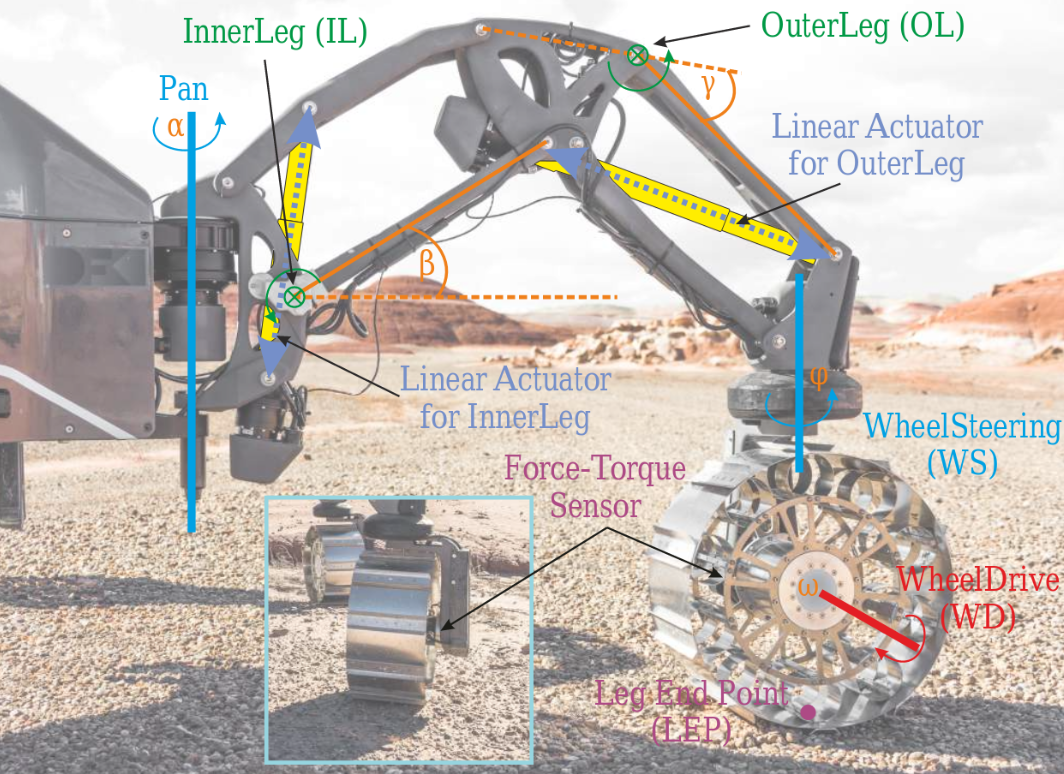
\includegraphics[width=0.6\linewidth]{sections/locomotion-power-draws/images/sherpatt-actively-articulated-suspension-sytem.png}\\
  \caption[SherpaTT actively articulated suspension system]
          {SherpaTT actively articulated suspension system, taken from \citeother{Cordes2018}.}
  \label{fig:sherpatt-actively-articulated-suspension-system}
\end{figure}

\clearpage
Lack of motor optimisation as well as lower gravity and pressure on Mars permit the assumption that, given similar topology traversals, measured propulsion power draws are greater than those that would be observed on a Martian environment. This assumption is further supported when considering that SherpaTT's velocities during power draw measurements were much greater than what has been achieved on present and past Mars rover missions.

Available datasets from the Mars analogue field test campaign cover two flat surface runs and three steep upslope terrain runs. From the two upslope runs, the dataset with the worst-case maximum and mean propulsion power draw was used as the worst-case scenario. Hereafter, all mention of SherpaTT power draws will reference measurements included in these datasets. Measured power draws fluctuate due to slips, skids, noise, and other unknown imperfections. To ease readability, local minima, maxima, and media lines have been traced for all power plot figures.

\subsection{Flat Terrain Traverse}
\label{sec:PowerBudget:PropulsionPowerBudget:FlatTerrainTraverse}
Both \ac{MER} and \ac{MSL} rovers are each equipped with a total of 10 propulsion motors to drive their Rocker-Bogie passive suspension system: six to rotate the wheels and four to steer them \citeother{Novak2005} \citeother{Lakdawalla2018}. The \ac{MER} rovers needed approximately \SI{100}{\watt} to drive \citeother{MERRoverEnergy}. Equation \ref{eq:InitialPropulsionPowerEstimate} was used for to determine an initial SherpaTT propulsion power draw using a single \ac{MER} wheel power draw as an estimation unit:

\begin{align}
  \label{eq:InitialPropulsionPowerEstimate}
  P_{prop}^{sherpatt} &= \frac{P_{prop}^{mer}}{N_{wheels}^{mer}} \times N_{wheels}^{sherpatt} \times \left(1 +\frac{P_{susp}^{sherpatt}}{P_{prop}^{sherpatt}}\right) \\
           &= \frac{100}{6} \times 4 \times 1.17\\
           &= \SI{78}{\watt}
\end{align}


where $P_{prop}$ is the total propulsion power, $P_{susp}$ is the total suspension power, $N_{wheels}$ is the number of wheels, and $P_{susp}^{sherpatt} / P_{prop}^{sherpatt}$ is the suspension system's share of the total propulsion power. For the latter, a worst-case 17\% was taken from \citeother{Cordes2018} for data collected from a flat terrain outdoor setting.

The propulsion power draws measured for SherpaTT on flat surface runs are shown in Figure \ref{fig:plot:sherpatt-flat-terrain-power-draw}. These measurements are summarised in Table \ref{tab:sherpatt-flat-terrain-global-minimum-maximum-and-medium-power-draws}. To eliminate power draw fluctuations from the analysis, only local media values were considered. Local media were selected rather than the worst-case local maxima on the basis of the assumptions made in Section \ref{sec:PowerBudget:PropulsionPowerBudget}. For flat terrain traverses, a worst-case maximum power draw of \SI{74}{\watt} is observed in close accordance with the initial estimate obtained from Equation \ref{eq:InitialPropulsionPowerEstimate}.
\pagebreak

\begin{figure}[h]
\captionsetup[subfigure]{justification=centering}
\vspace{-2ex}
	\centering
    %% setup sizes
    \setlength{\subfigureWidth}{0.50\textwidth}
    \setlength{\graphicsHeight}{80mm}
    %% kill hyper-link highlighting
    \hypersetup{hidelinks=true}%
    %% the figures
    \begin{subfigure}[t]{\subfigureWidth}
        \centering
        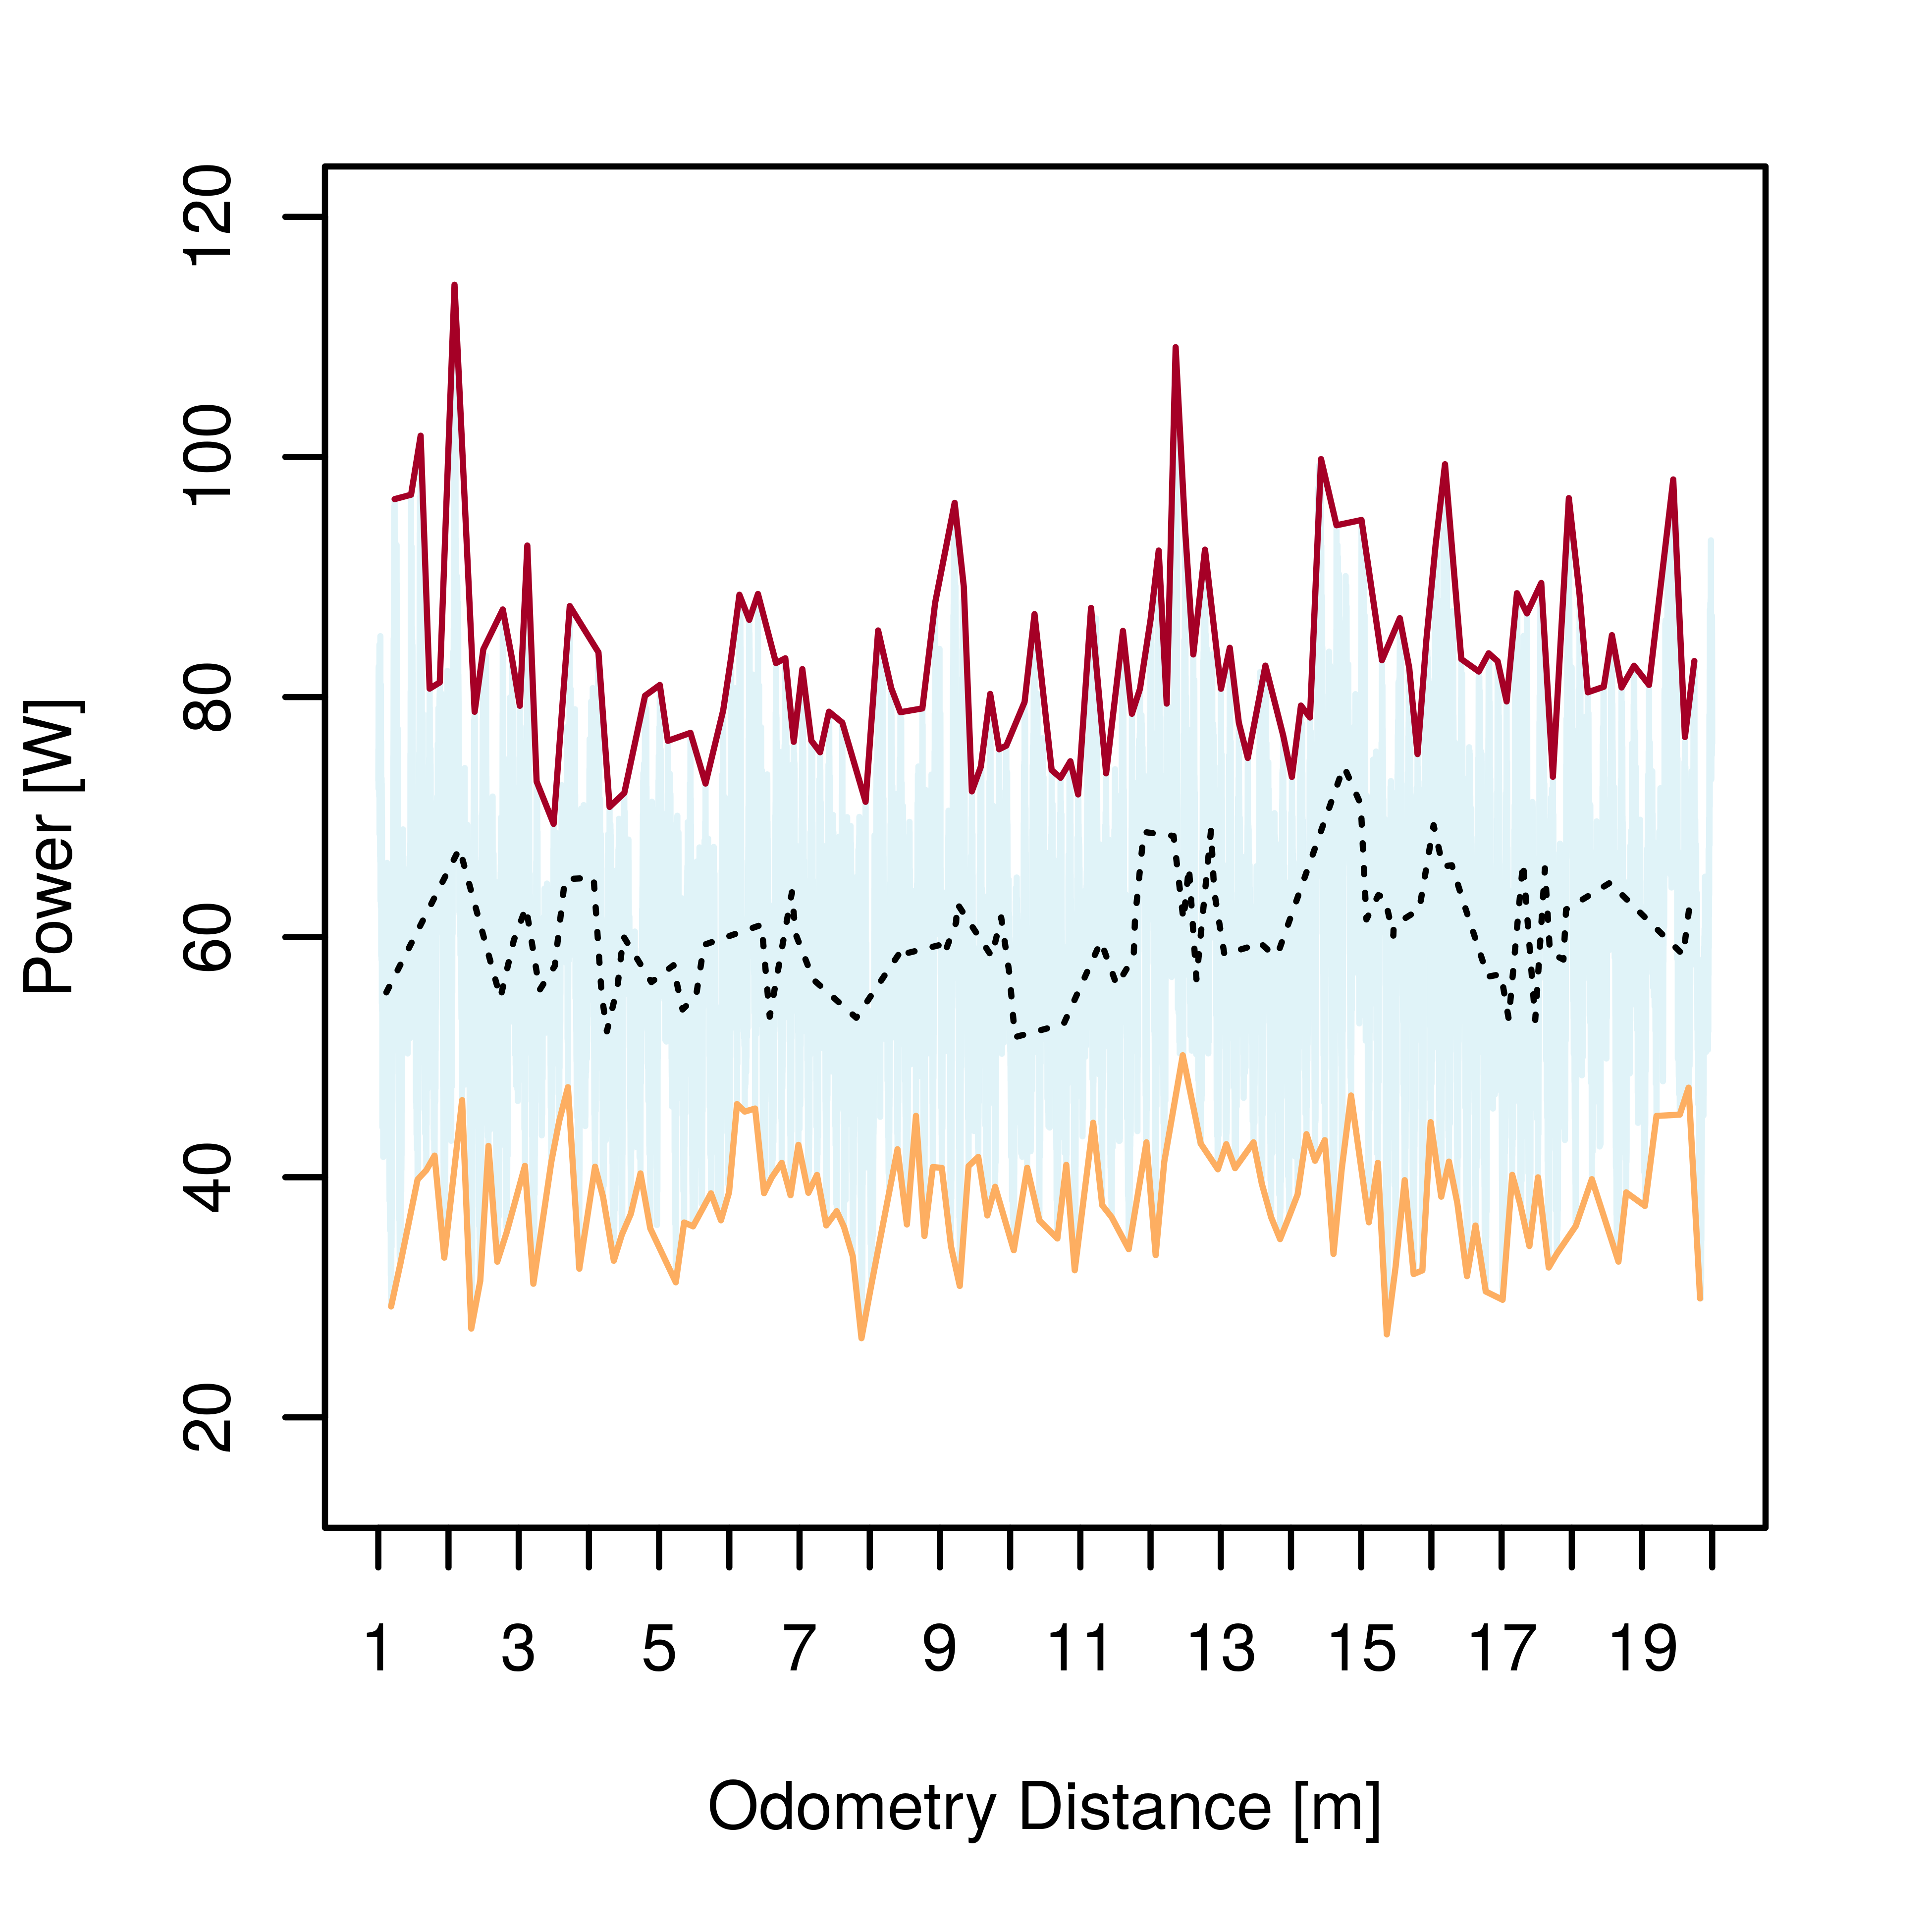
\includegraphics[height=\graphicsHeight]{sections/locomotion-power-draws/plots/locomotion-power-draw-on-flat-terrain-1.png}
        \subcaption{Run \#1}
        \label{fig:plot:sub:sherpatt-flat-terrain-power-draw-1}
    \end{subfigure}\hfill
    \begin{subfigure}[t]{\subfigureWidth}
        \centering
        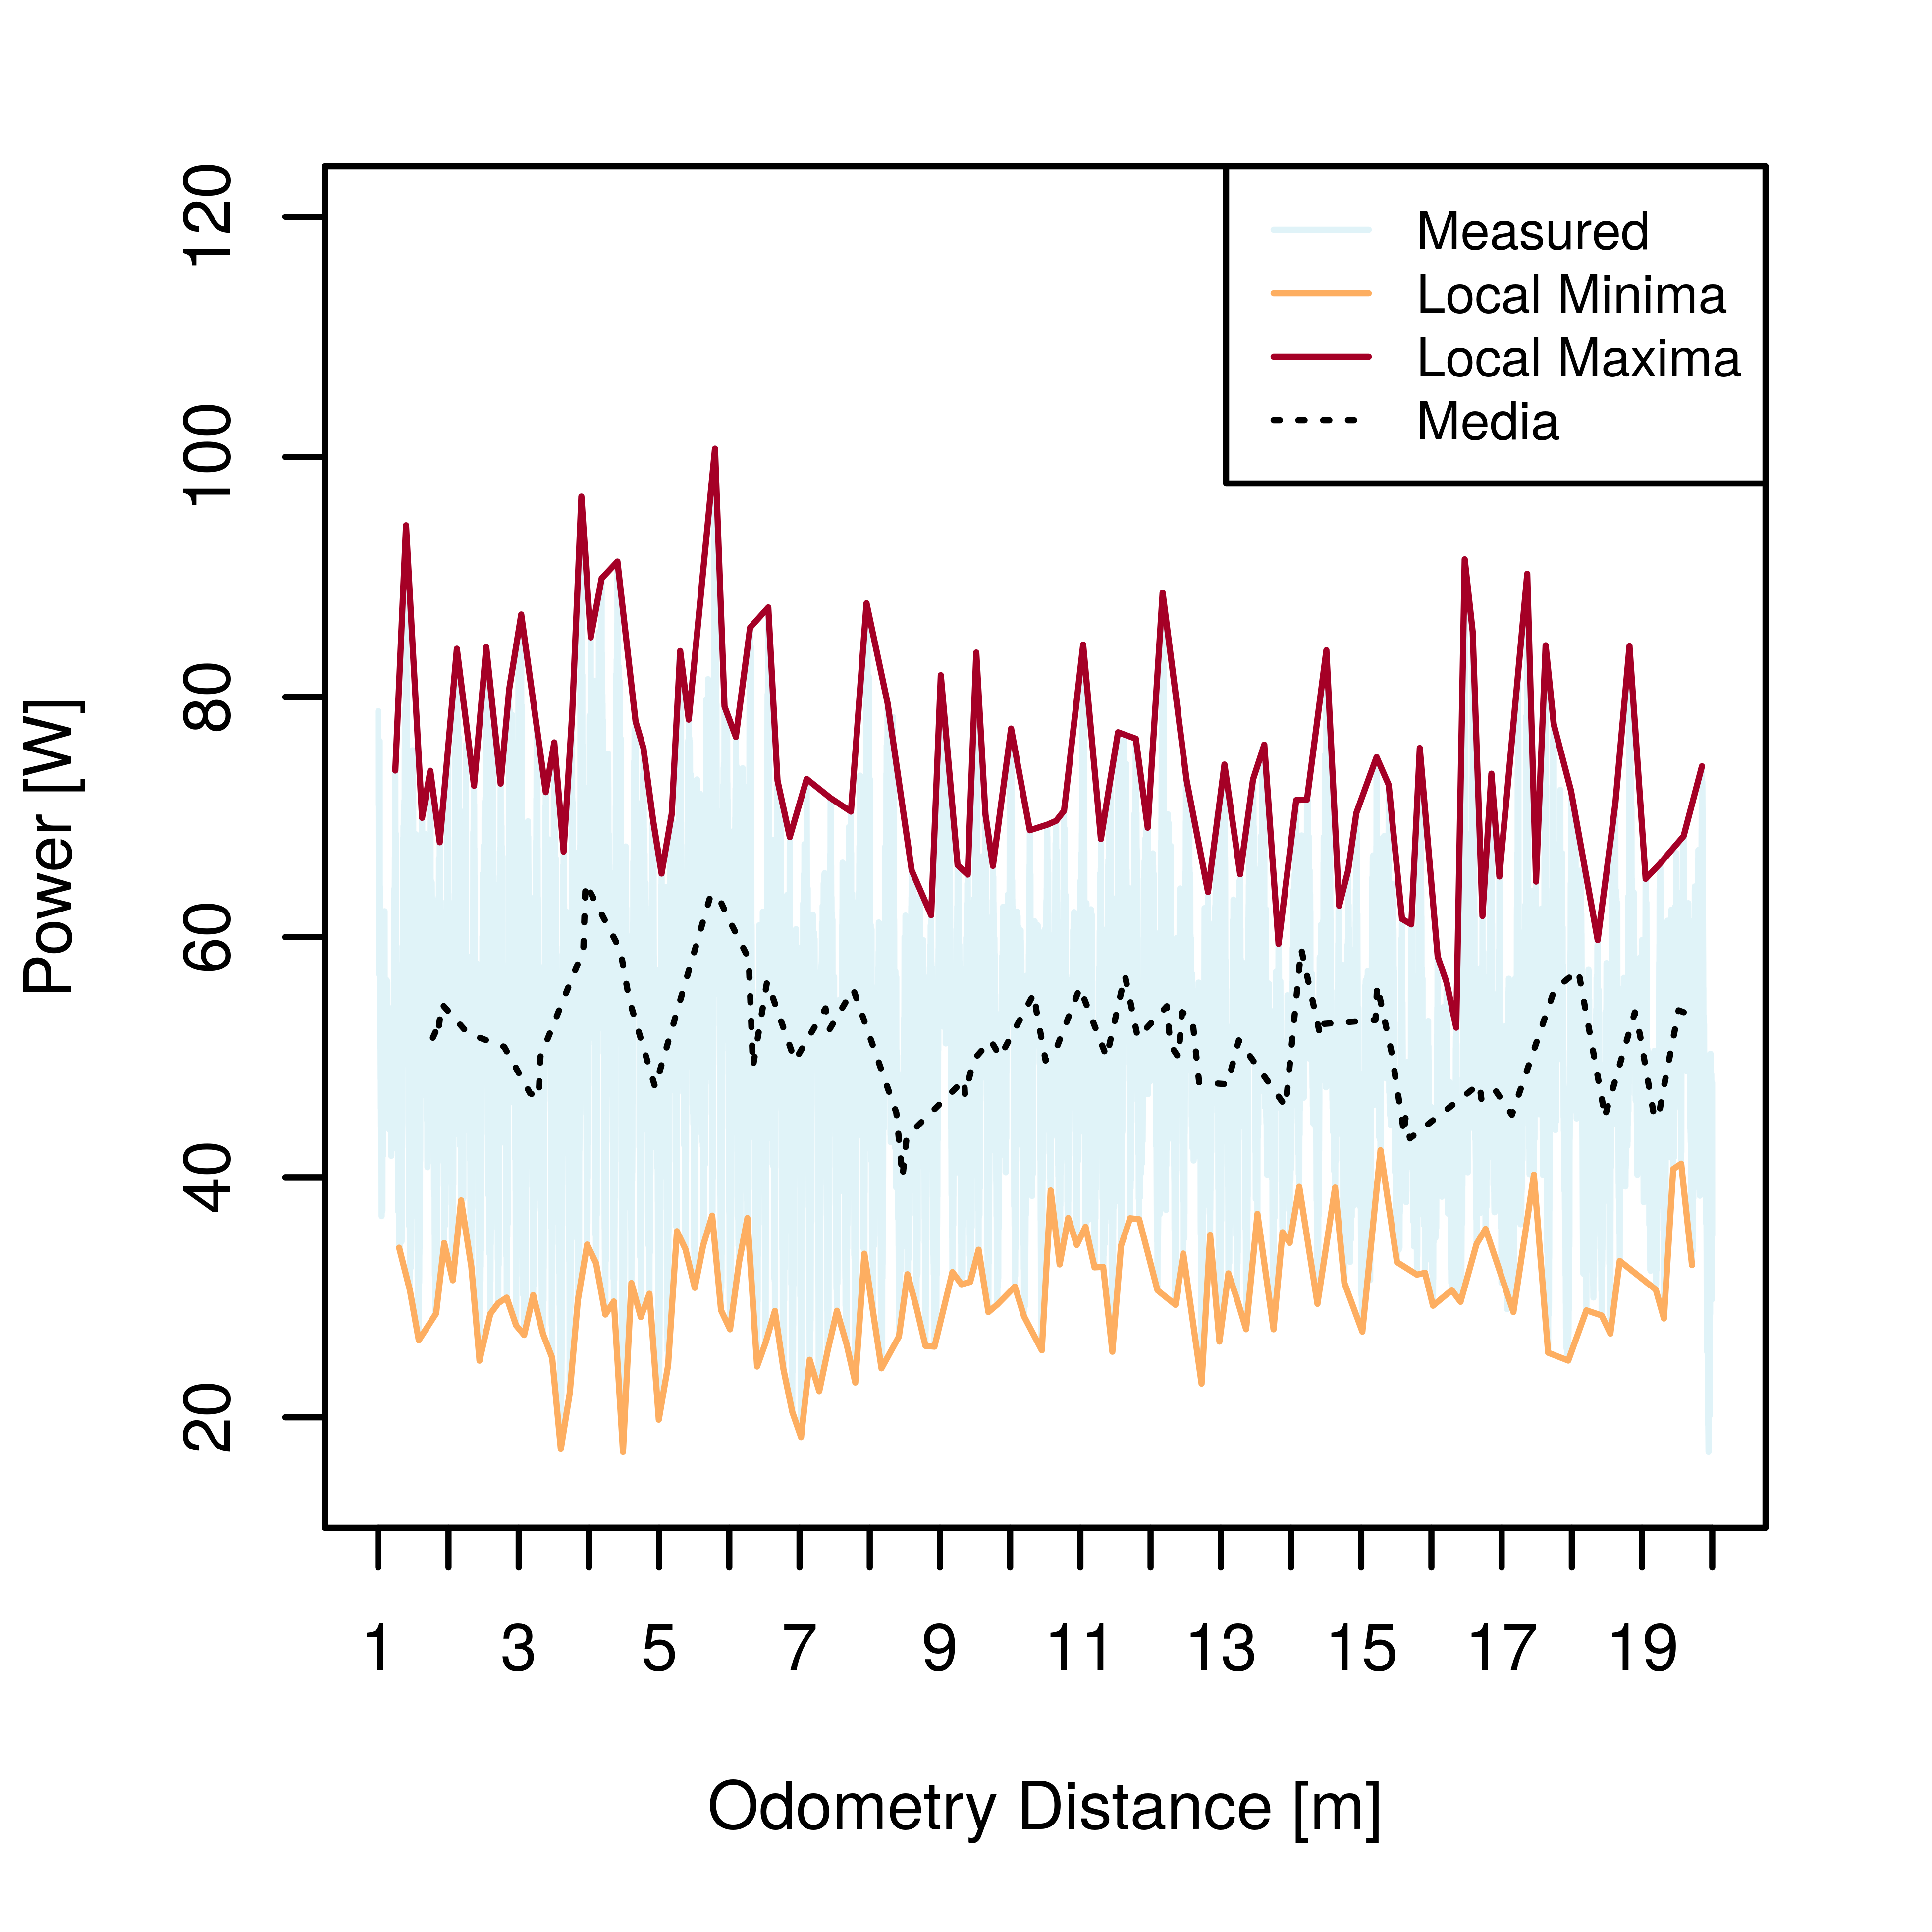
\includegraphics[height=\graphicsHeight]{sections/locomotion-power-draws/plots/locomotion-power-draw-on-flat-terrain-2.png}
  		\subcaption{Run \#2}
		\label{fig:plot:sub:sherpatt-flat-terrain-power-draw-2}
	\end{subfigure}\\[0.8ex]
    \caption[Propulsion power draw for a flat terrain traverse during SherpaTT Mars analogue field tests in Utah]
            {Propulsion power draw for a flat terrain traverse during SherpaTT Mars analogue field tests in Utah.}
    \label{fig:plot:sherpatt-flat-terrain-power-draw}
\vspace{-2ex}
\end{figure}



\begin{table}[h]
\centering
\caption{Global minimum, maximum, and medium of traced local minima, maxima, and media for SherpaTT flat terrain propulsion power draw lines.}
\label{tab:sherpatt-flat-terrain-global-minimum-maximum-and-medium-power-draws}
\begin{tabular}{llccc}
\cline{3-5}
\multicolumn{2}{l|}{\multirow{2}{*}{}} & \multicolumn{3}{c|}{\textbf{Power Draw {[}W{]}}} \\ \cline{3-5}
\multicolumn{2}{l|}{} & \multicolumn{1}{c|}{\textbf{\begin{tabular}[c]{@{}c@{}}Global Minimum\end{tabular}}} & \multicolumn{1}{c|}{\textbf{\begin{tabular}[c]{@{}c@{}}Global Maximum\end{tabular}}} & \multicolumn{1}{c|}{\textbf{\begin{tabular}[c]{@{}c@{}}Global Media\end{tabular}}} \\ \hline
\multicolumn{1}{|c|}{\multirow{4}{*}{\textbf{Run \#1}}} & \multicolumn{1}{l|}{\textbf{Measured}} & \multicolumn{1}{c|}{27} & \multicolumn{1}{c|}{114} & \multicolumn{1}{c|}{60} \\ \cline{2-5}
\multicolumn{1}{|c|}{} & \multicolumn{1}{l|}{\textbf{Local Minima}} & \multicolumn{1}{c|}{27} & \multicolumn{1}{c|}{50} & \multicolumn{1}{c|}{38} \\ \cline{2-5}
\multicolumn{1}{|c|}{} & \multicolumn{1}{l|}{\textbf{Local Maxima}} & \multicolumn{1}{c|}{69} & \multicolumn{1}{c|}{114} & \multicolumn{1}{c|}{83} \\ \cline{2-5}
\multicolumn{1}{|c|}{} & \multicolumn{1}{l|}{\textbf{Local Media}} & \multicolumn{1}{c|}{52} & \multicolumn{1}{c|}{74} & \multicolumn{1}{c|}{61} \\ \hhline{|=|=|=|=|=|}
\multicolumn{1}{|l|}{\multirow{4}{*}{\textbf{Run \#2}}} & \multicolumn{1}{l|}{\textbf{Measured}} & \multicolumn{1}{c|}{17} & \multicolumn{1}{c|}{101} & \multicolumn{1}{c|}{51} \\ \cline{2-5}
\multicolumn{1}{|l|}{} & \multicolumn{1}{l|}{\textbf{Local Minima}} & \multicolumn{1}{c|}{17} & \multicolumn{1}{c|}{42} & \multicolumn{1}{c|}{30} \\ \cline{2-5}
\multicolumn{1}{|l|}{} & \multicolumn{1}{l|}{\textbf{Local Maxima}} & \multicolumn{1}{c|}{52} & \multicolumn{1}{c|}{101} & \multicolumn{1}{c|}{74} \\ \cline{2-5}
\multicolumn{1}{|l|}{} & \multicolumn{1}{l|}{\textbf{Local Media}} & \multicolumn{1}{c|}{40} & \multicolumn{1}{c|}{64} & \multicolumn{1}{c|}{52} \\ \hline
 &  & \multicolumn{1}{l}{} & \multicolumn{1}{l}{} & \multicolumn{1}{l}{} \\
 &  & \multicolumn{1}{l}{} & \multicolumn{1}{l}{} & \multicolumn{1}{l}{}
\end{tabular}
\end{table}


\pagebreak
\subsection{Upslope Terrain Traverse}
\label{sec:PowerBudget:PropulsionPowerBudget:UpslopeTerrainTraverse}
Propulsion power draws on a steep uplsope were measured along an approximately \SI{16}{\meter} track and are shown Figure \ref{fig:plot:sub:sherpatt-disaggregated-upslope-terrain-power-draw-locomotion}. An initial estimate of \SI{132}{\watt} was obtained using Equation \ref{eq:InitialPropulsionPowerEstimate} with a worst case 98\% suspension system's share of the total propulsion power taken from \citeother{Cordes2018} for data collected from a steep slope outdoor setting.

The drive and suspension power draw components are shown in Figures \ref{fig:plot:sub:sherpatt-disaggregated-upslope-terrain-power-draw-drive} and \ref{fig:plot:sub:sherpatt-disaggregated-upslope-terrain-power-draw-suspension}, respectively.

\begin{figure}[h]
\captionsetup[subfigure]{justification=centering}
\vspace{-2ex}
	\centering
    %% setup sizes
    \setlength{\subfigureWidth}{0.32\textwidth}
    \setlength{\graphicsHeight}{50mm}
    %% kill hyper-link highlighting
    \hypersetup{hidelinks=true}%
    %% the figures
	\begin{subfigure}[t]{\subfigureWidth}
        \centering
        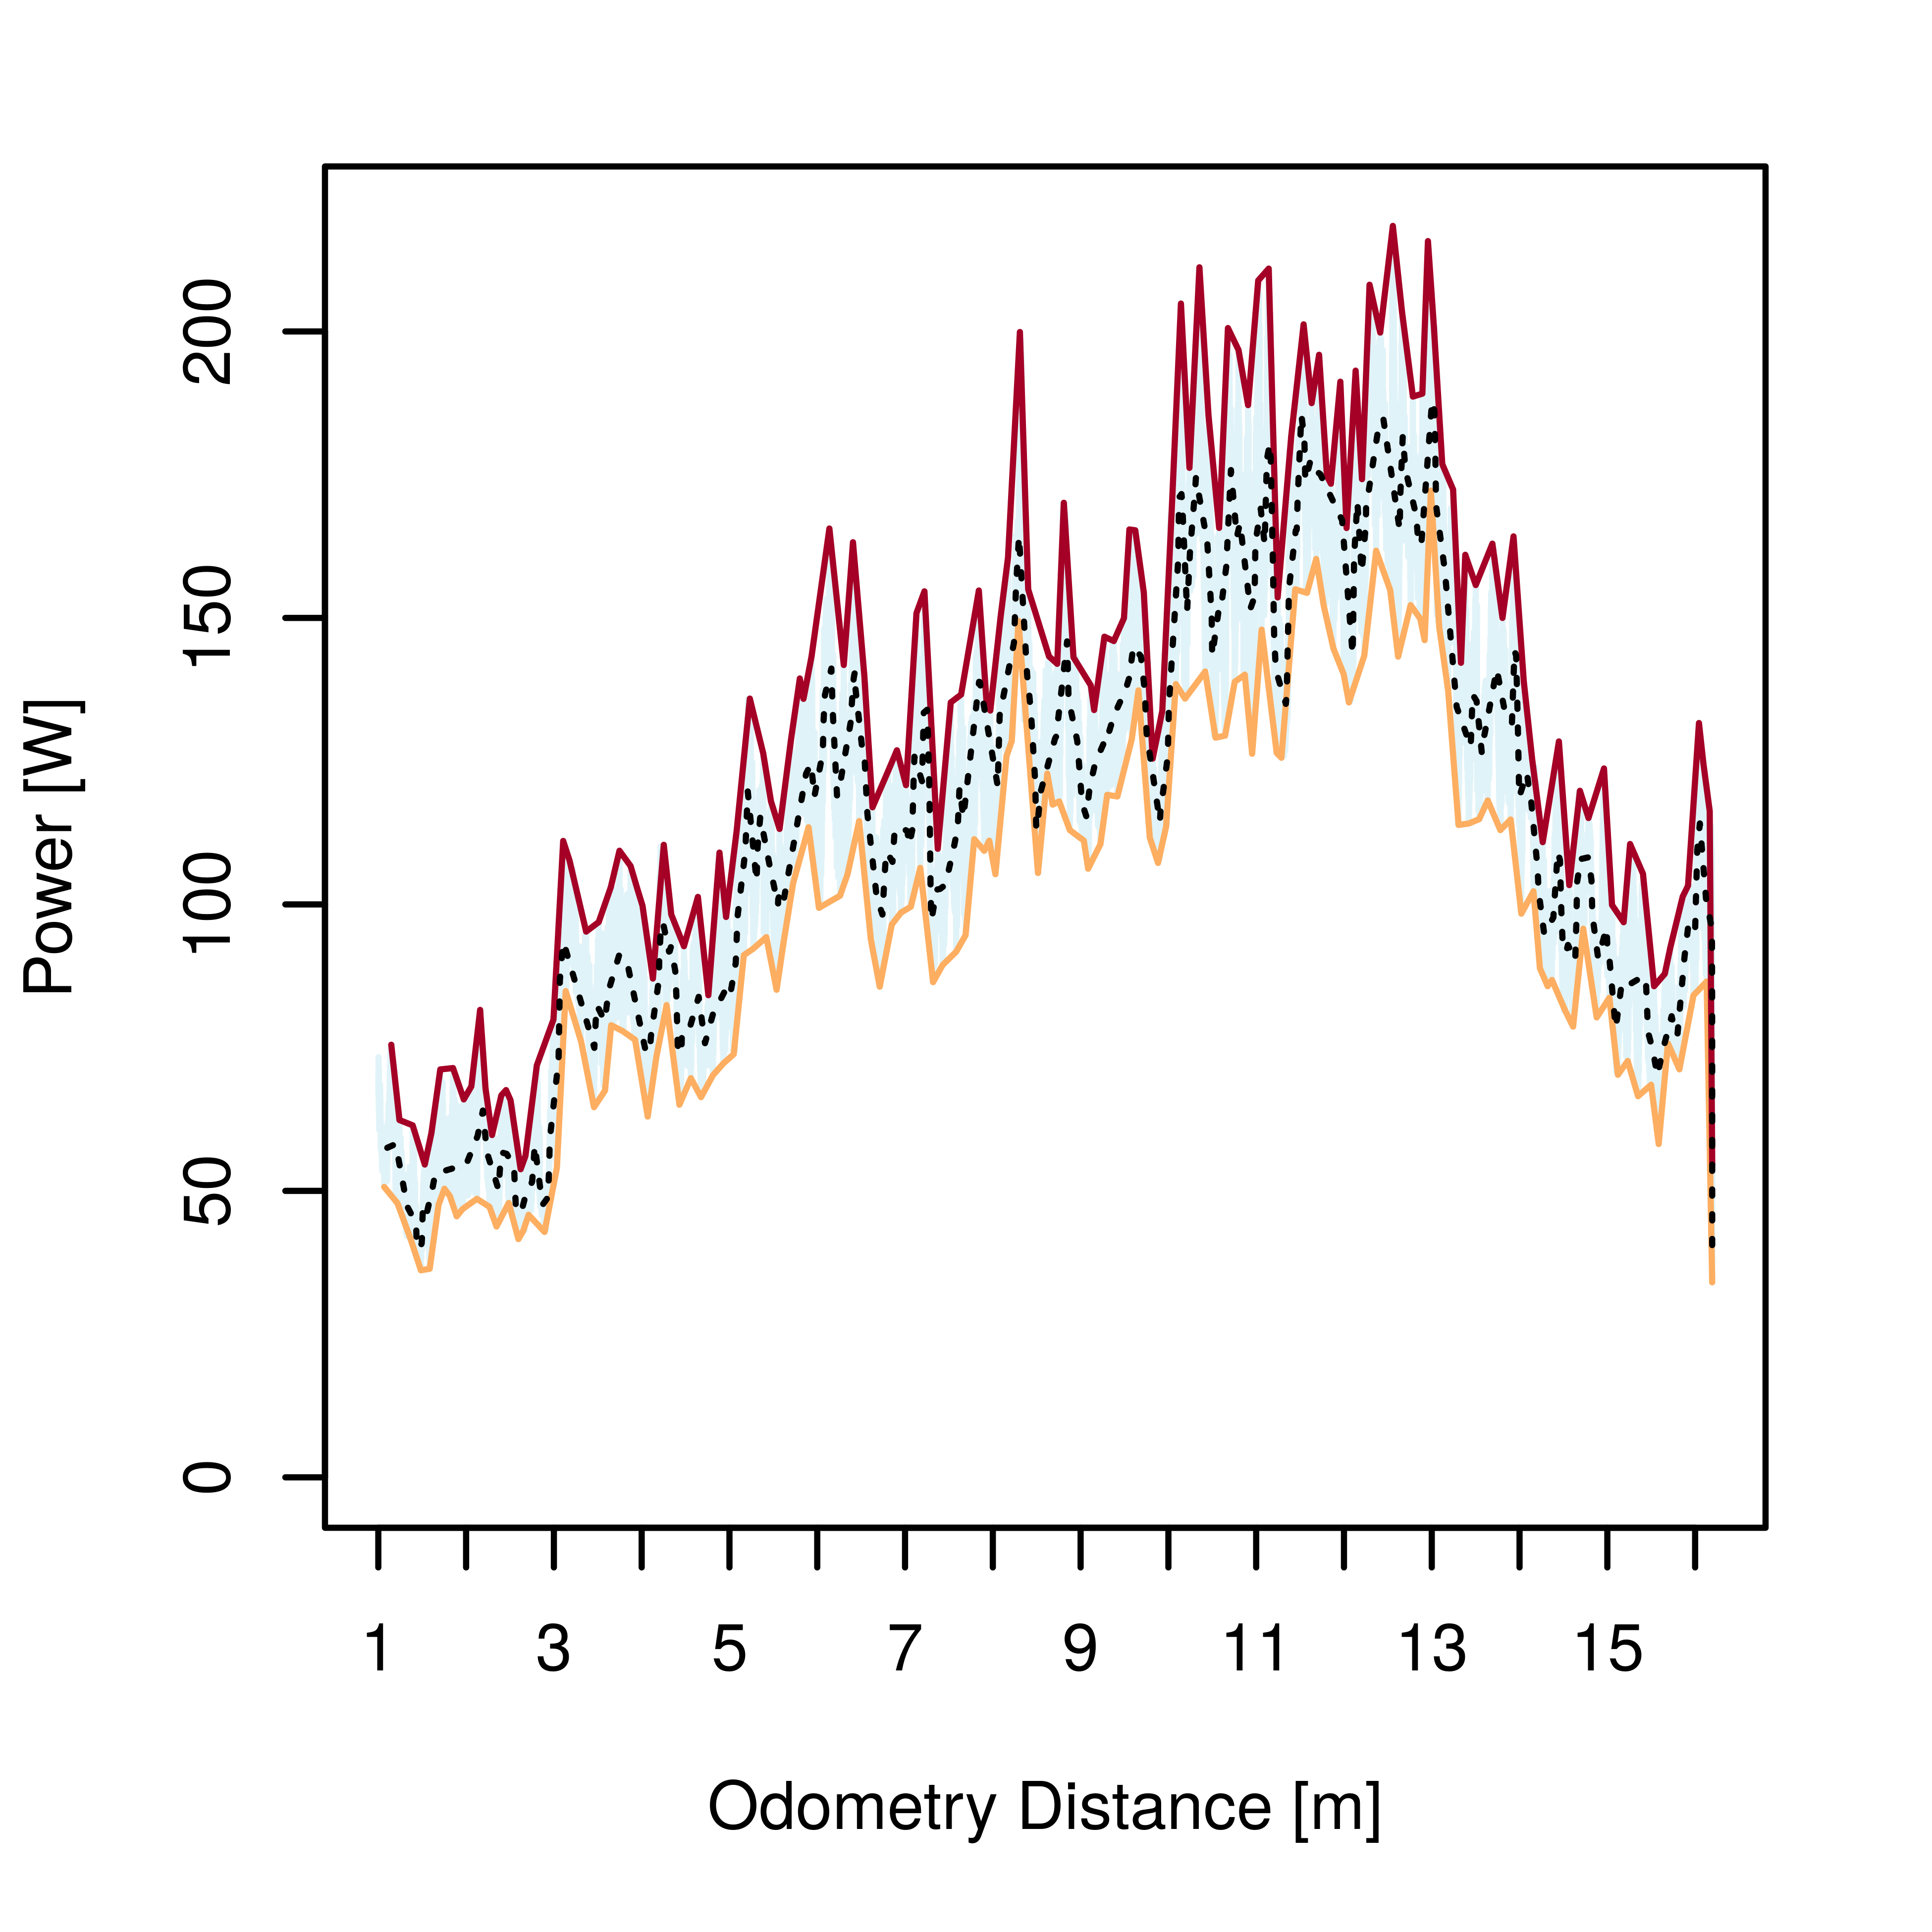
\includegraphics[height=\graphicsHeight]{sections/locomotion-power-draws/plots/locomotion-power-draw-on-upslope-terrain.png}
  		\subcaption{Propulsion}
		\label{fig:plot:sub:sherpatt-disaggregated-upslope-terrain-power-draw-locomotion}
	\end{subfigure}\hfill
	\begin{subfigure}[t]{\subfigureWidth}
        \centering
        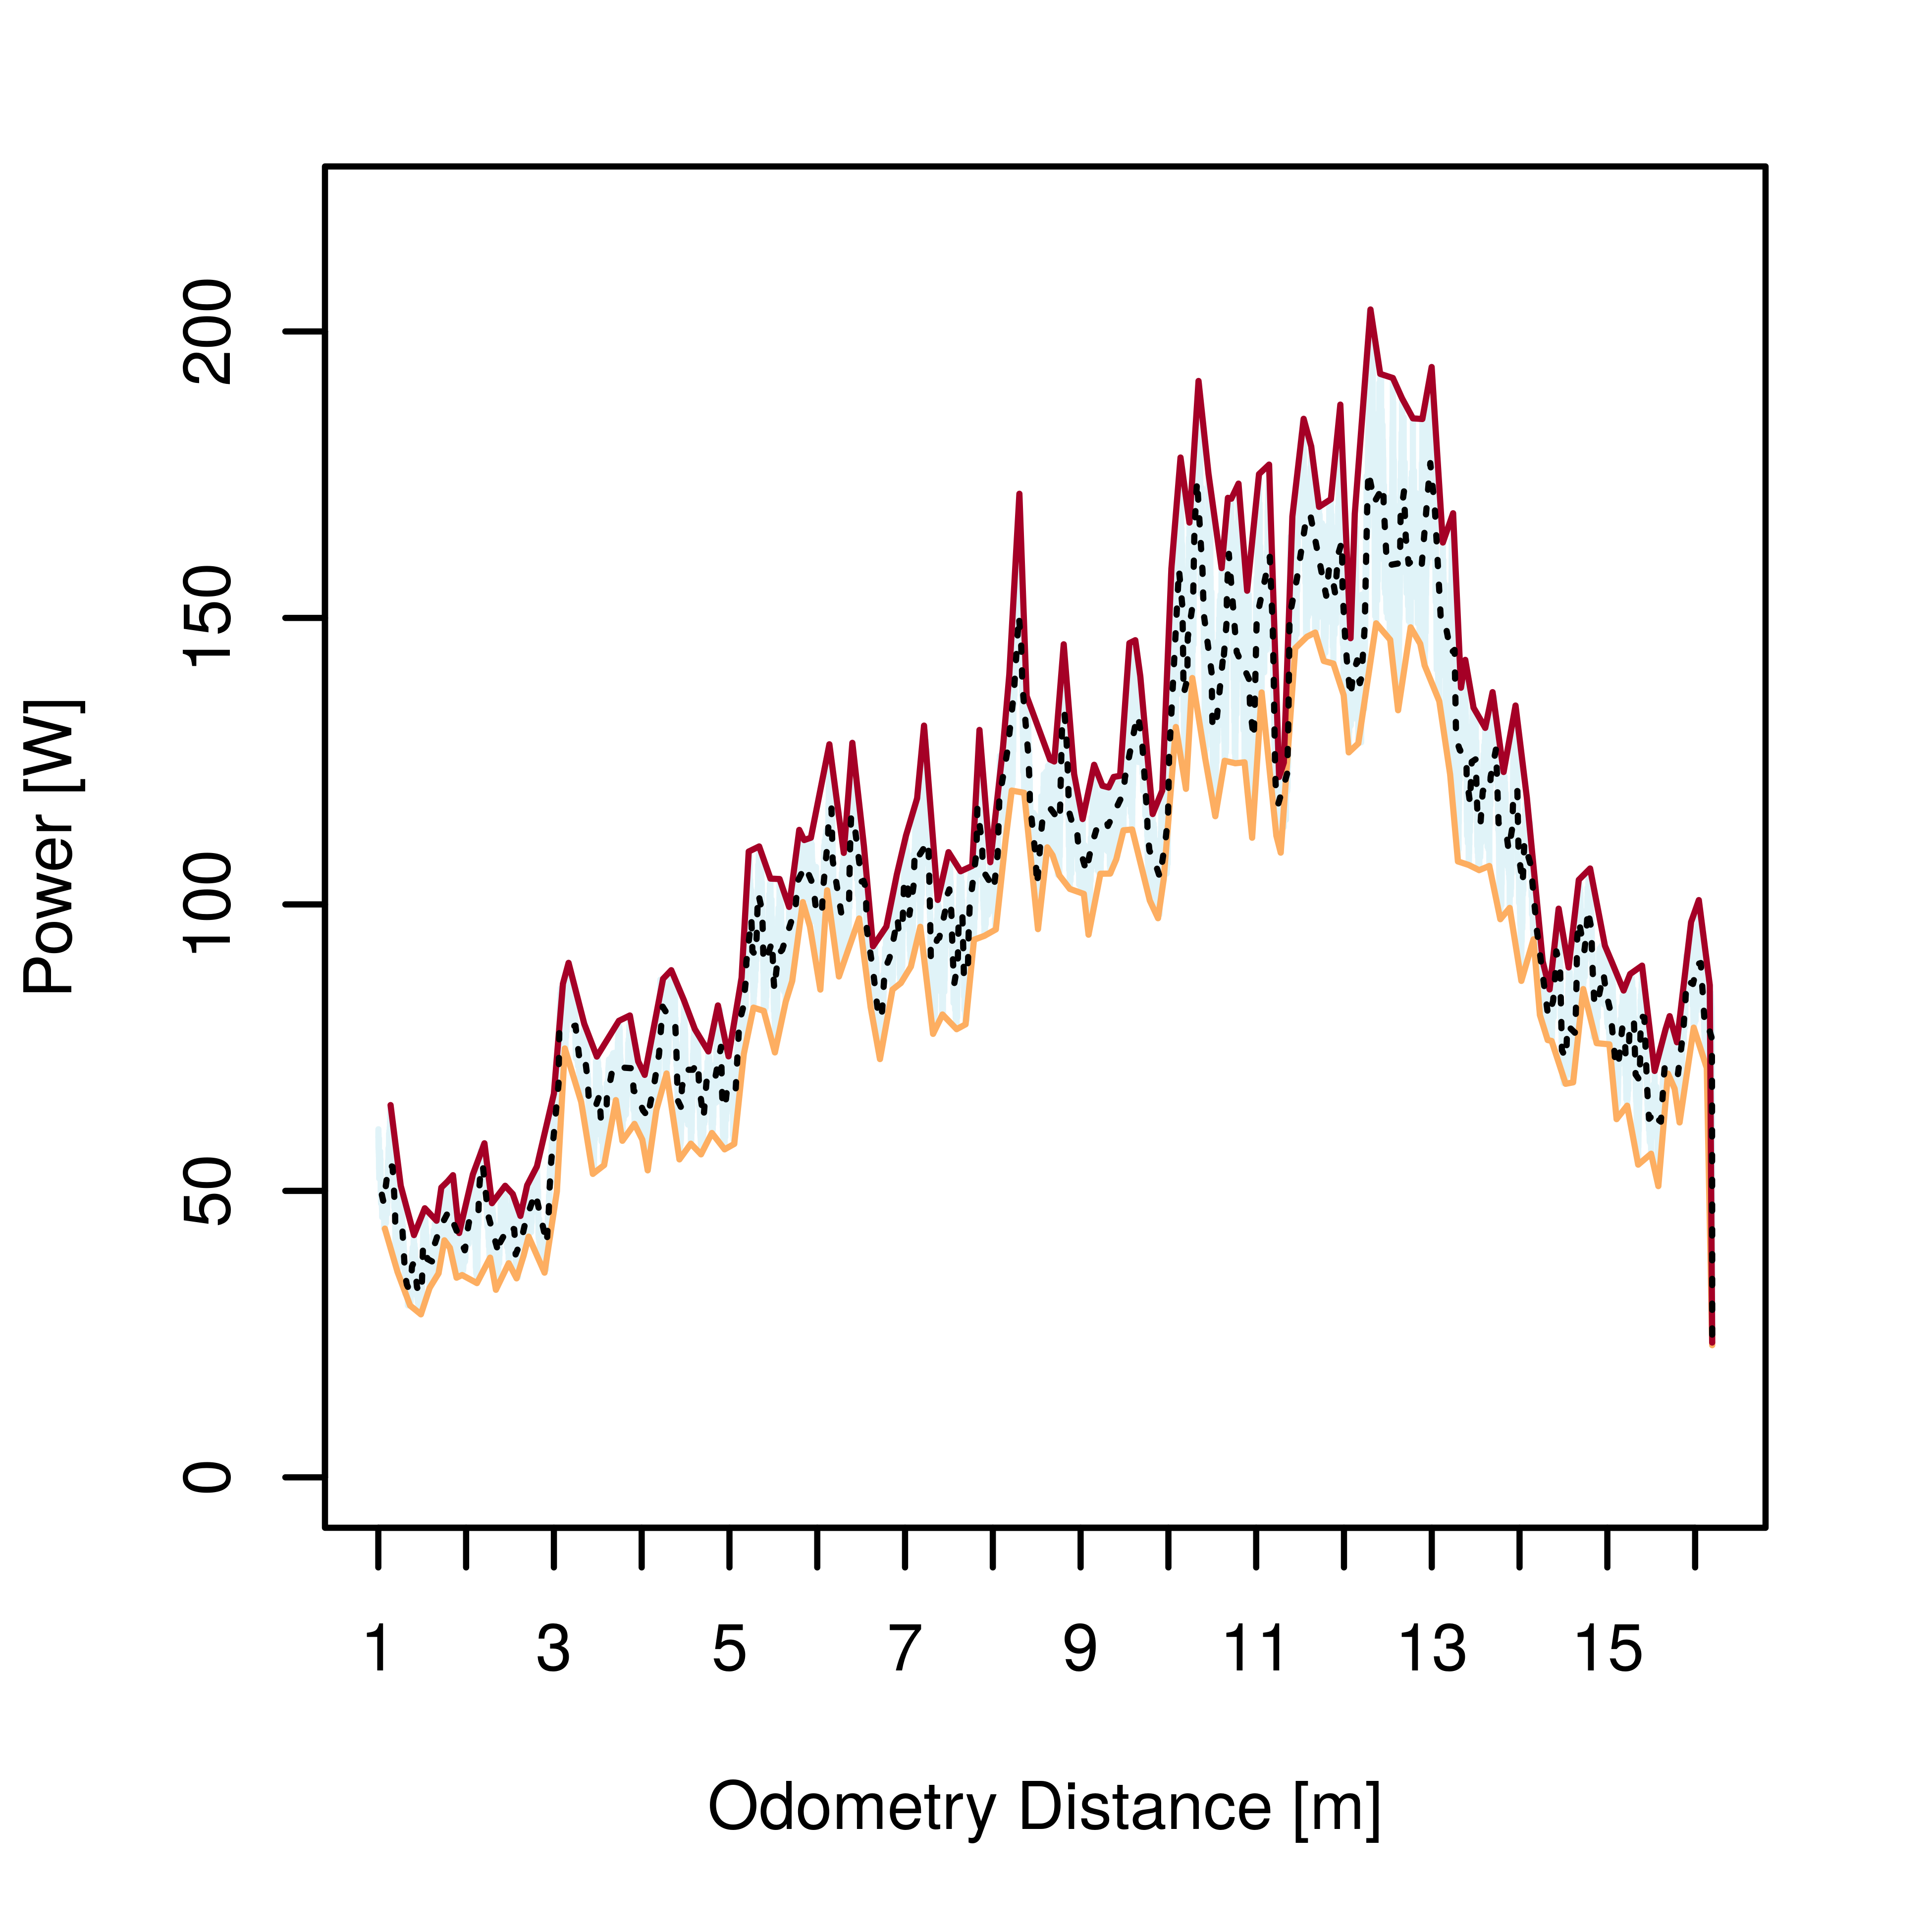
\includegraphics[height=\graphicsHeight]{sections/locomotion-power-draws/plots/drive-power-draw-on-upslope-terrain.png}
  		\subcaption{Drive}
		\label{fig:plot:sub:sherpatt-disaggregated-upslope-terrain-power-draw-drive}
	\end{subfigure}\hfill
    \begin{subfigure}[t]{\subfigureWidth}
        \centering
        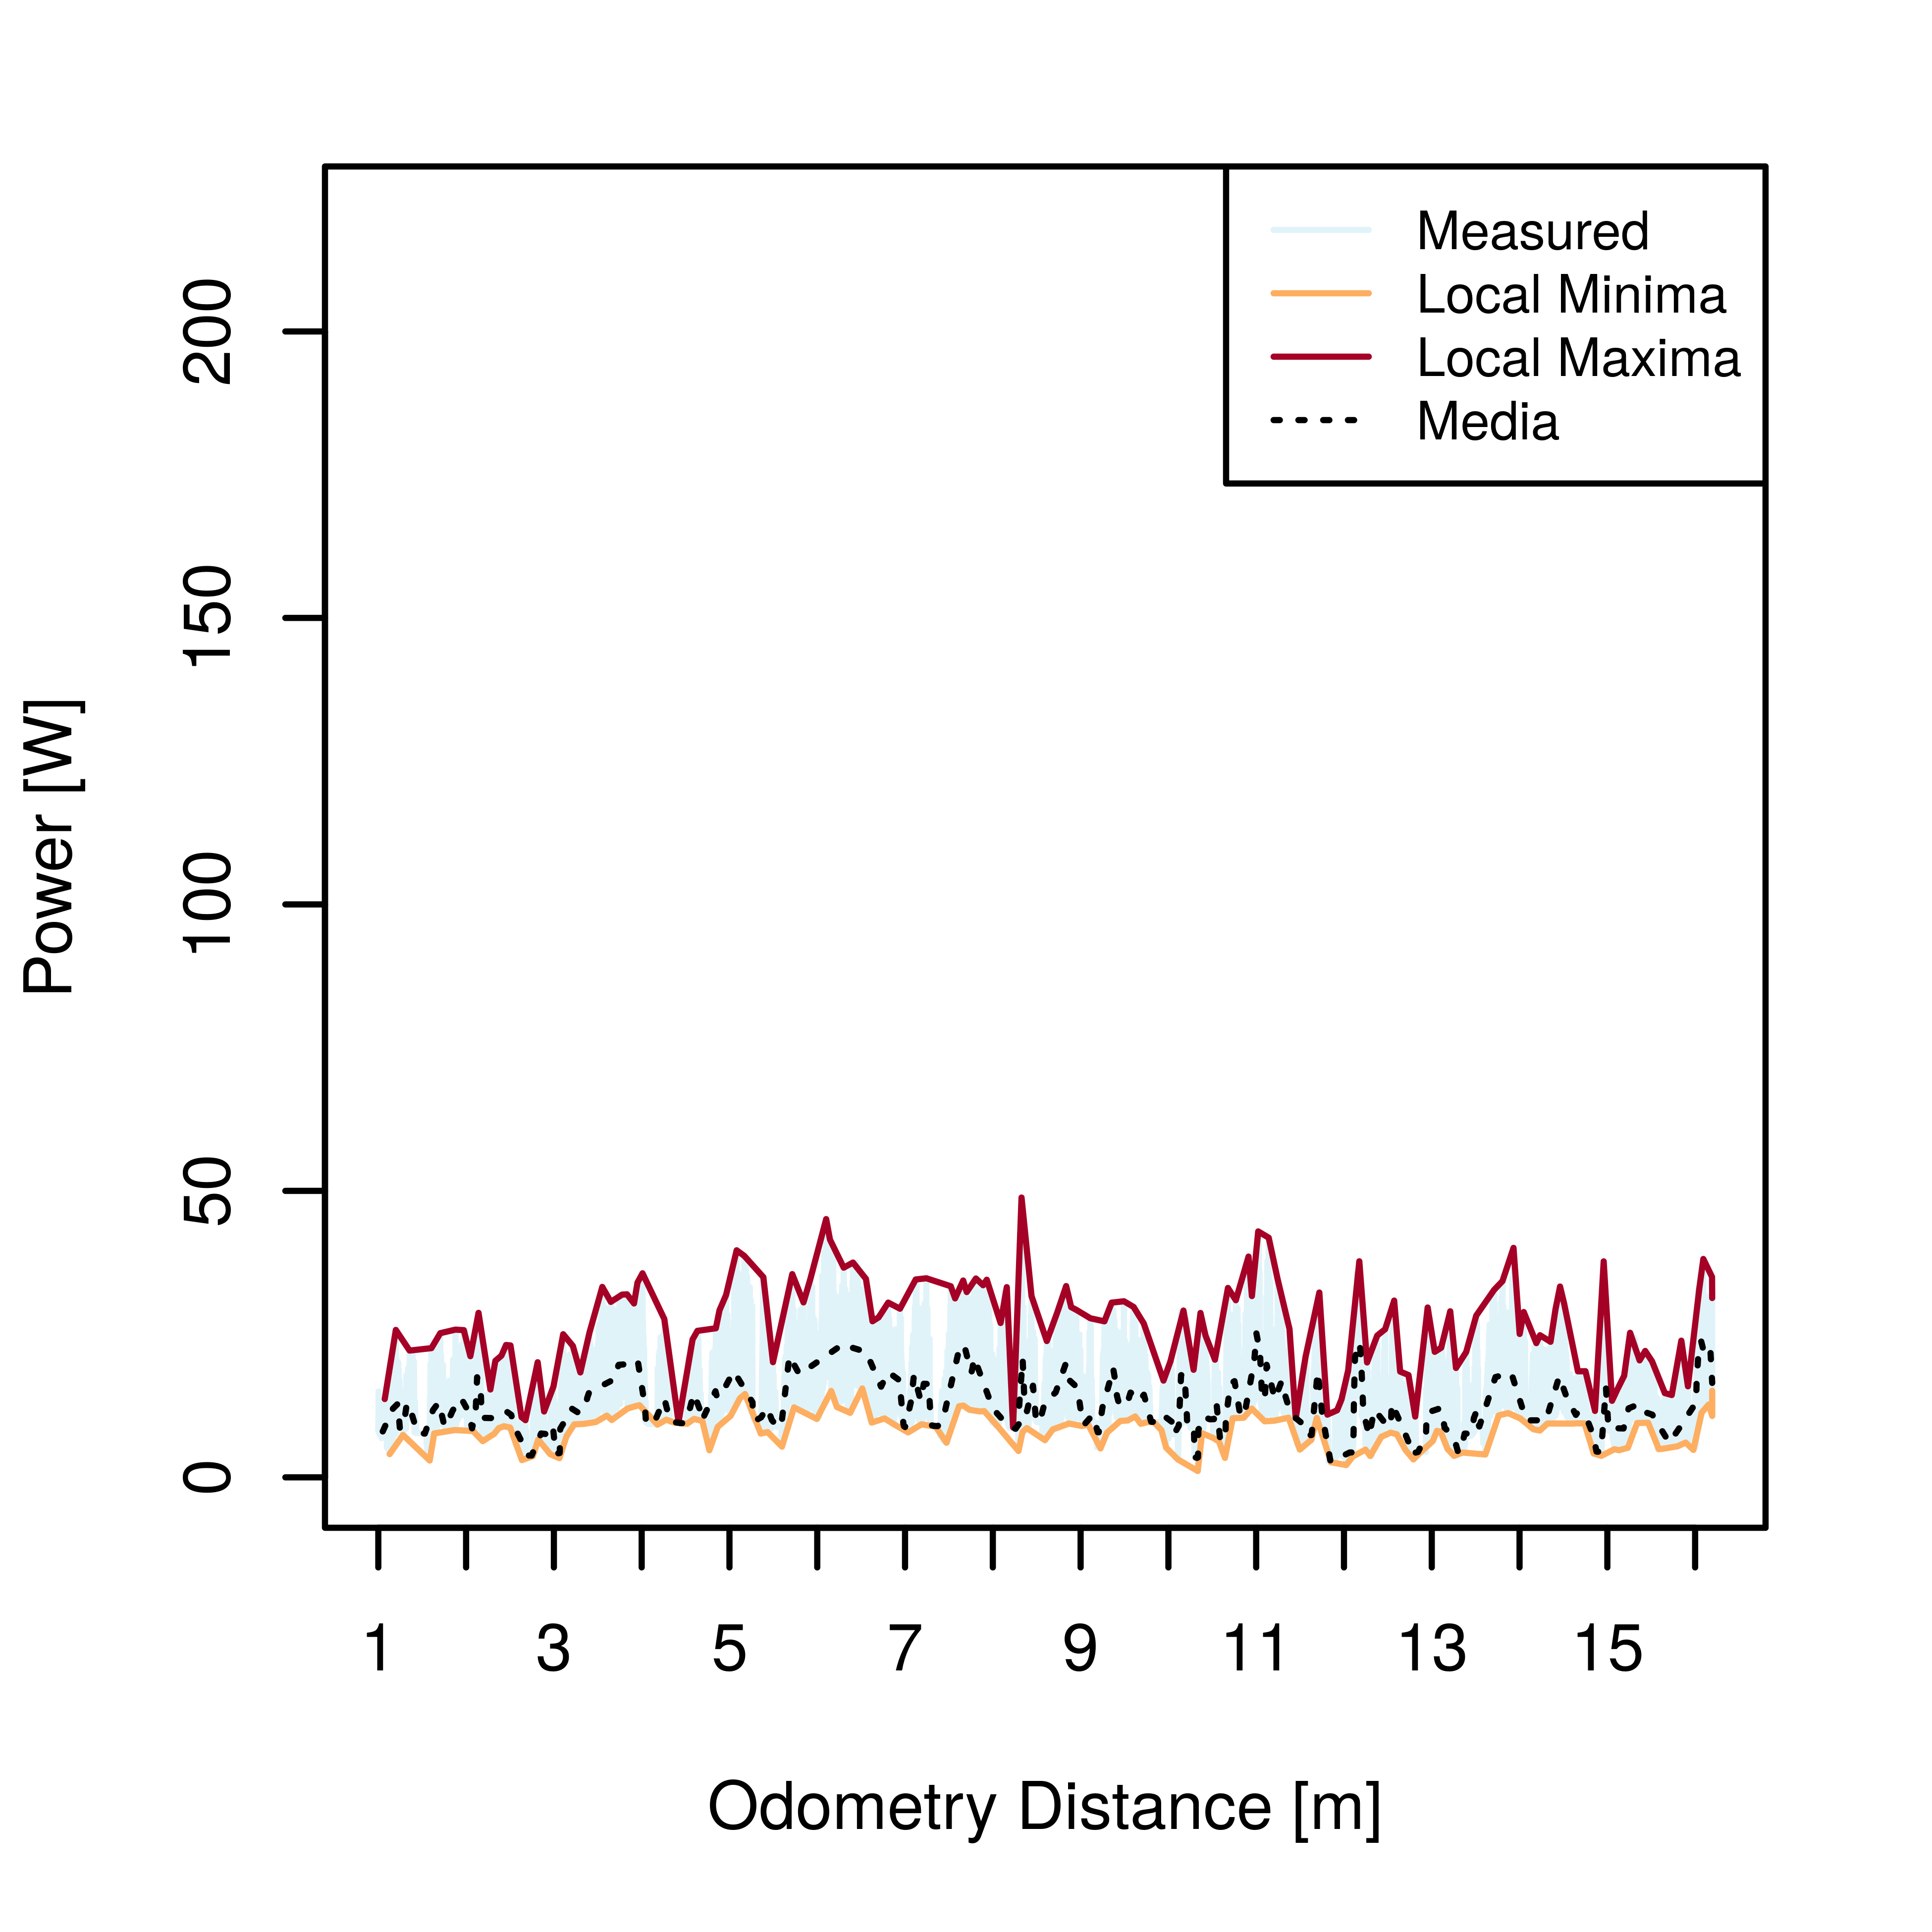
\includegraphics[height=\graphicsHeight]{sections/locomotion-power-draws/plots/suspension-power-draw-on-upslope-terrain.png}
  		\subcaption{Suspension}
		\label{fig:plot:sub:sherpatt-disaggregated-upslope-terrain-power-draw-suspension}
	\end{subfigure}\\[0.8ex]
    \caption[Disaggregated measurements of power draw for upslope terrain traverse during SherpaTT Mars analogue field tests in Utah]
            {Disaggregated measurements of power draw for upslope terrain traverse during SherpaTT Mars analogue field tests in Utah.}
    \label{fig:plot:sherpatt-disaggregated-upslope-terrain-power-draw}
\vspace{-2ex}
\end{figure}

An uplsope traverse has no discernable effect on the suspension power draw, however; there is a clear gradual increase in the drive power draw. The global maximum, minimum, and medium of the traced local minima, maxima, and media power draw lines are presented in Table \ref{tab:sherpatt-upslope-terrain-global-minimum-maximum-and-medium-power-draws}.

\begin{table}[h]
\centering
\caption{Global minimum, maximum, and medium of traced local minima, maxima, and media for SherpaTT upslope terrain traverse propulsion power draw lines.}
\label{tab:sherpatt-upslope-terrain-global-minimum-maximum-and-medium-power-draws}
\begin{tabular}{l|c|c|c|}
\cline{2-4}
\multicolumn{1}{c|}{\multirow{2}{*}{\textbf{}}} & \multicolumn{3}{c|}{\textbf{Power Draw {[}W{]}}} \\ \cline{2-4}
\multicolumn{1}{c|}{} & \textbf{\begin{tabular}[c]{@{}c@{}}Global Minimum\end{tabular}} & \textbf{\begin{tabular}[c]{@{}c@{}}Global Maximum\end{tabular}} & \textbf{\begin{tabular}[c]{@{}c@{}}Global Media\end{tabular}} \\ \hline
\multicolumn{1}{|l|}{\textbf{Measured}} & 34 & 218 & 114 \\ \hline
\multicolumn{1}{|l|}{\textbf{Local Minima}} & 34 & 172 & 98 \\ \hline
\multicolumn{1}{|l|}{\textbf{Local Maxima}} & 54 & 218 & 133 \\ \hline
\multicolumn{1}{|l|}{\textbf{Local Media}} & 40 & 188 & 18 \\ \hline
\end{tabular}
\end{table}


Figure \ref{fig:plot:sherpatt-upslope-terrain-power-draw} overlaps the propulsion local media power draws with the tackled slope angles. The steepest slope angle was \SI{28}{\degree} for an average of \SI{17.52}{\degree}. Slope angle increase are consistently followed by power draw spikes, i.e. at approximately 3, 4, 5, 6, 8, and 9 meters in the odometry measurements. Inversely, slope angle decreases were followed by power draws troughs at approximately 11, 13, 14, and 16 meters.

\clearpage
\begin{figure}[h]
  \centering
  \hypersetup{linkcolor=captionTextColor}
  \includegraphics[width=0.8\linewidth]{sections/locomotion-power-draws/plots/minima-locomotion-power-draws-on-upslope-terrain.png}\\
  \caption[Mean Propulsion power draw for an upslope terrain traverse during SherpaTT Utah field test campaign.]
          {Mean Propulsion power draw for an upslope terrain traverse during SherpaTT Utah field test campaign.}
  \label{fig:plot:sherpatt-upslope-terrain-power-draw}
\end{figure}

The power draws trough following the slope angle change from \SI{28}{\degree} to \SI{20}{\degree} at the \SI{11}{\meter} mark is subsequently followed by an unusual power draw increase and fluctuation. These measurements were discarded as they are outliers with respect to the power draw responses for the slope angle descreases that followed.

Table \ref{tab:sherpatt-upslope-terrain-local-media-measurement-summary} summarises the minimum, maximum, and mean local media propulsion power draws that were measured for different slope angles. Discarding the outlier measurements subsequent to the slope angle change from \SI{28}{\degree} to \SI{20}{\degree} at the \SI{11}{\meter} to \SI{13}{\meter} portion of the track, the maximum mean local media propulsion power draw is \SI{146}{\watt}, which is close to the initial estimate given by Equation \ref{eq:InitialPropulsionPowerEstimate}.

\begin{table}[h]
\centering
\caption{SherpaTT mean propulsion power draw measurements for different slope sections}
\label{tab:sherpatt-upslope-terrain-local-media-measurement-summary}
\begin{tabular}{cc|c|c|c|}
\cline{3-5}
\multicolumn{1}{l}{} & \multicolumn{1}{l|}{} & \multicolumn{3}{c|}{\textbf{Power {[}W{]}}} \\ \hline
\multicolumn{1}{|l|}{\textbf{Distance {[}m{]}}} & \multicolumn{1}{l|}{\textbf{Slope Angle {[}deg{]}}} & \multicolumn{1}{l|}{\textbf{Minimum}} & \multicolumn{1}{l|}{\textbf{Maximum}} & \multicolumn{1}{l|}{\textbf{Mean}} \\ \hline
\multicolumn{1}{|c|}{\textbf{1 $<$ x $\leq$ 3}} & 10 & 40 & 64 & 51 \\ \hline
\multicolumn{1}{|c|}{\textbf{3 $<$ x $\leq$ 4}} & 11 & 73 & 93 & 85 \\ \hline
\multicolumn{1}{|c|}{\textbf{4 $<$ x $\leq$ 5}} & 15 & 74 & 87 & 83 \\ \hline
\multicolumn{1}{|c|}{\textbf{5 $<$ x $\leq$ 6}} & 16 & 85 & 125 & 107 \\ \hline
\multicolumn{1}{|c|}{\textbf{6 $<$ x $\leq$ 7}} & 28 & 98 & 141 & 123 \\ \hline
\multicolumn{1}{|c|}{\textbf{7 $<$ x $\leq$ 8}} & 22 & 97 & 139 & 116 \\ \hline
\multicolumn{1}{|c|}{\textbf{8 $<$ x $\leq$ 9}} & 25 & 113 & 164 & 133 \\ \hline
\multicolumn{1}{|c|}{\textbf{9 $<$ x $\leq$ 11}} & 28 & 114 & 176 & 146 \\ \hline
\multicolumn{1}{|c|}{\textbf{11 $<$ x $\leq$ 13}} & 20 & 135 & 188 & 167 \\ \hline
\multicolumn{1}{|c|}{\textbf{13 $<$ x $\leq$ 14}} & 15 & 119 & 123 & 145 \\ \hline
\multicolumn{1}{|c|}{\textbf{14 $<$ x $\leq$ 16}} & 10 & 70 & 186 & 94 \\ \hline
\end{tabular}
\end{table}


\pagebreak
\section{Power Budget}
\label{sec:PowerBudget:PowerBudget}
The duration of  due to the worst-case daytime length differences between Iani Chaos and Ismenius Cavus, which are located at different planetary latitudes. The latter is located at a higher latitude, in the northern hemisphere, and will thus receive less daylight during the winter season.

\subsection{Flat Traverse}
\label{sec:PowerBudget:PowerBudget:FlatTraverse}

Power and duration values for \textit{DTE Communication}, \textit{Science Stop}, and \textit{Hibernation} modes were taken from \ac{CDF} and assigned to the Reference Sols presented in Section \ref{sec:ReferenceSols:ReferenceSols}, these are shown in Table ref{tab:ReferenceSolsPowerBudget}. Propulsion power for the \textit{Traverse} modes were replaced by values based on power draw estimates in Sections \ref{sec:PowerBudget:PropulsionPowerBudget:FlatTerrainTraverse} and \ref{sec:PowerBudget:PropulsionPowerBudget:UpslopeTerrainTraverse}, that is \SI{75}{\watt} for flat terrain traverses and \SI{150}{\watt} for upslope terrain traverses up to \SI{30}{\degree} inclination. The \textit{Optimal Pose} mode's power draw was estimated at \SI{75}{\watt} based on the rover's flat terrain propulsion power draw and is etimated to take up to \SI{10}{\minute} to execute.

\begin{table}[h]
\footnotesize
\centering
\caption{Best- and worst-case Traverse Sol power budget for optimal pose at mission site locations during a clear sky day (tau=0.4). P is Power [W], t is duration [min], and E is energy [Wh].}
\label{tab:power-budget-traverse-sol-tau-0p4}
\begin{tabular}{lc|c|c|c|c|c|c|c|c|}
\cline{3-10}
 & \multicolumn{1}{l|}{} & \multicolumn{4}{c|}{\textbf{Iani Chaos}} & \multicolumn{4}{c|}{\textbf{Ismenius Cavus}} \\ \cline{3-10}
 & \multicolumn{1}{l|}{\begin{tabular}[c]{@{}c@{}}\\ \\ \end{tabular}} & \multicolumn{2}{c|}{\textbf{$H^{wc}_{L_{s}=\SI{78}{\degree}, \beta=\SI{10}{\degree}}$}} & \multicolumn{2}{c|}{\textbf{$H^{bc}_{L_{s}=\SI{234}{\degree}, \beta=\SI{10}{\degree}}$}} & \multicolumn{2}{c|}{\textbf{$H^{wc}_{L_{s}=\SI{274}{\degree}, \beta=\SI{10}{\degree}}$}} & \multicolumn{2}{c|}{\textbf{$H^{bc}_{L_{s}=\SI{134}{\degree}, \beta=\SI{10}{\degree}}$}} \\ \hline
\multicolumn{1}{|c|}{\textbf{Mode}} & \textbf{$P$} & \textbf{$t_{1}$} & \textbf{$E_{1} = Pt_{1}$} & \textbf{$t_{2}$} & \textbf{$E_{2}$} & \textbf{$t_{3}$} & \textbf{$E_{3}$} & \textbf{$t_{4}$} & \textbf{$E_{4}$} \\ \hline
\multicolumn{1}{|l|}{\textbf{Idle - Day}} & 29 & 499 & 241 & 197 & 95 & 403 & 195 & 110 & 53 \\ \hline
\multicolumn{1}{|l|}{\textbf{DTE Communication}} & 52 & 35 & 30 & 35 & 30 & 35 & 30 & 35 & 30 \\ \hline
\multicolumn{1}{|l|}{\textbf{Traverse}} & 113 & 109 & 205 & 424 & 799 & 66 & 124 & 604 & 1138 \\ \hline
\multicolumn{1}{|l|}{\textbf{Science Stop - Short}} & 60 & 60 & 60 & 60 & 60 & 60 & 60 & 60 & 60 \\ \hline
\multicolumn{1}{|l|}{\textbf{Optimal Pose}} & 75 & 10 & 13 & 10 & 13 & 10 & 13 & 10 & 13 \\ \hline
\multicolumn{1}{|l|}{\textbf{Idle - Night}} & 20 & 727 & 242 & 714 & 238 & 866 & 289 & 621 & 207 \\ \hhline{|=|=|=|=|=|=|=|=|=|=|}
\multicolumn{2}{|r|}{\textbf{Total}} & \textbf{1440} & \textbf{791} & \textbf{1440} & \textbf{1235} & \textbf{1440} & \textbf{711} & \textbf{1440} & \textbf{1501} \\ \hline
\multicolumn{2}{|r|}{\textbf{Total +20\% system margin}} & - & \textbf{949} & - & \textbf{1482} & - & \textbf{853} & - & \textbf{1801} \\ \hline
\end{tabular}
\end{table}




\subsection{Upslope Traverse}
\label{sec:PowerBudget:PowerBudget:UpslopeTraverse}

\subsection{Hibernation}
\label{sec:PowerBudget:PowerBudget:Hibernation}

\section{Summary and Conclusion}
\label{sec:PowerBudget:SummaryAndConclusion}
